%===================================================================================================
%  Chapter : 磁束密度
%  説明    : 磁束密度の概念を導入する
%===================================================================================================
%======================================================================
%  Section
%======================================================================
    \section{磁束密度に関するローレンツ力}
    \begin{mycomment}
        世の中には,電気的な力と似たような,しかし,それとは異なる力が
        存在する.それは,磁気的な力である.磁石が及ぼす力が,その代表
        的な例であることは,誰もが承知しているところだ.
        ここでは,磁気と電荷の関係について説明しよう.
    \end{mycomment}

    \begin{mysmallsec}{磁束密度の存在を示す現象}
        磁石付近において,正電荷を帯びた物体がある速度で横切ると,
        その物体はその速度の方向を曲げられるような力を受ける.
        イメージは,図\ref{fig:Lorentz_Force_image}である
            \footnote{
                図中の \textbf{磁束密度} という語彙があるが,これは
                磁石の向きを表したものであると,考えてもらいたい.
                磁束密度の定義などの詳細は,後述する.
                イメージはこれで十分である.
            }.
        \begin{figure}[hbt]
            \begin{tabular}{cc}
                \begin{minipage}{0.5\hsize}
                    \begin{center}
                        \includegraphicsdouble{Lorentz_Force_image1.pdf}

                        (A) 正電荷
                    \end{center}
                \end{minipage}
                \begin{minipage}{0.5\hsize}
                    \begin{center}
                        \includegraphicsdouble{Lorentz_Force_image2.pdf}

                        (B) 負電荷
                    \end{center}
                \end{minipage}
            \end{tabular}
                        \caption{磁束密度に関するローレンツ力}
                        \label{fig:Lorentz_Force_image}
        \end{figure}

        磁石に近づく前は,直線的な運動(等速直線運動)をしていたの
        だけど,磁石に近づいたら,その運動方向が換えられてしまうので
        ある.当然,人間が引っ張ったわけではない.磁石の存在により,
        運動方向が変化するのである.図\ref{fig:Lorentz_Force_image}(A)で
        は,下に曲げられている様子を描いた.このような状況であれば,
        正電荷を帯びた物体ならば,常に下向きに運動方向が変わる.つまり,
        磁石から生じる磁界
            \footnote{
                磁界:後に,\textbf{磁束密度} という呼び方に言い改める.
                しかし,ここでは,小学生の頃から使い慣れている語彙を
                優先して,「磁界」と記述した.イメージすることが最優
                先であるので.
            }
        の向きに対して,右回転するように曲がるのである.ということは
        もちろん,磁界の向きが図\ref{fig:Lorentz_Force_image}(A)とは
        逆向きであれば,物体は上方向に曲げられることになる.

        運動する物体が負電荷の場合(図\ref{fig:Lorentz_Force_image}(B)),
        曲げられる方向は,正電荷の場合と逆向きで,上の方に曲がる.

        また,図には描いてないが,磁界の向きが逆(S極付近を通過する場合)
        の場合,曲げられる向きは,正電荷が曲げられる向きと反対方向である.

        以上のように,電気量を帯びた物体が磁極付近を通過するときには,
        その運動方向が,磁極の向きに対し右回りするように,曲げられる.
        物体の運動方向の変化は,その速度の変化を意味していて,つまりは
        加速度が生じたということになる.加速度が生じるのは,物体が何らかの力
        を受けたということである.このような力のことを,
        \textbf{磁束密度に関するローレンツ力} とよぶ
            \footnote{
                Hendrik Antoon Lorentz(1853--1928, オランダ):
                ゼーマン(※1)とともに,\textbf{ゼーマン効果}
                (\pageref{subsec:ZeemanEffect}ページの\ref{subsec:ZeemanEffect}節を参照)
                を発見し,さらに
                理論付けを行ったことで,ノーベル物理学賞を授与されている.
                特殊相対性理論でよく使われる \textbf{ローレンツ変換} でも
                その名を残している.

                (※1)Pieter Zeeman(1865--1943, オランダ)
            }.
    \end{mysmallsec}

    \begin{mysmallsec}{定量化してみよう}
        数式で表してみよう.物体の回転を扱うのには,ベクトルの外積が
        便利である.実際,磁束密度に関するローレンツ力もベクトルの外積を用いて定義で
        きる.

        そのために,磁束密度という概念を定義したいのだけど,
        ここでちょっと発想の転換をしたい.
        今までは考えやすいように,磁界
            \footnote{
                使用している語彙が安定していないが,容赦してもらいたい.
                分かりやすく説明するため,未説明の語彙を不用意に使いた
                くない.未説明の語彙は,きちんと説明した後に,使用する
                こととしたい.それまでは,一般的に分かりやすいと思われる
                語彙や言い回しを使うことを許してほしい.
            }
        が存在する空間付近で,電気量を持った物体が磁束密度に関するローレンツ力を受け,
        進行方向が変わる,という説明をしてきた.しかし,ここで磁束密度という
        概念を定義するにあたり,視点をかえてみる.

        まず,最初に空間には“何も無い”と認識していると仮定しよう.
        ここに,わざと電気量をもった物体を適当な速度で等速直線運動
        させてみよう.本当に何もなければ,この物体は等速直線運動を
        続けるのみである.しかし,物体がある所から曲がったとしよう.
        当然,人間が外力を加えてわざと曲げたのではないとする.なぜ
        物体はそこから進行方向が変化してしまったのか.この疑問に答
        える為に,ここで \textbf{磁束密度} という考え方を導入するのであ
        る.最初に仮定していた“何も無い”空間は,実は“何も無い”のではなく,
        そこには,磁束密度が存在していたとするのである.この磁束密度により,
        電気量を帯びた物体が磁束密度に関するローレンツ力を受けて,進行方向を変化させられた
        と説明するのである.

        イメージは,図\ref{fig:MgField_def}のようである.
        まず,図\ref{fig:MgField_def}(A)を想定して電気量を帯びた
        物体を投げるのだが,“何もしていないのに”物体の進行方向が
        曲がってしまう.これを説明するため,そこには,“磁束密度が存在していた”
        とするのである(図\ref{fig:MgField_def}(B)).
        \begin{figure}[hbt]
            \begin{tabular}{cc}
                \begin{minipage}{0.5\hsize}
                    \begin{center}
                        \includegraphicsdouble{MgField_01.pdf}

                        (A) 何も無いはず!
                    \end{center}
                \end{minipage}
                \begin{minipage}{0.5\hsize}
                    \begin{center}
                        \includegraphicsdouble{MgField_02.pdf}

                        (B) 磁束密度の存在
                    \end{center}
                \end{minipage}
            \end{tabular}
                        \caption{磁束密度の存在}
                        \label{fig:MgField_def}
        \end{figure}

        ようやく,磁束密度に関するローレンツ力を数式で表す準備が整った.
        電気量 $q$ をもった物体(以降,電荷 $q$ と書く)が,
        速度 $\bv$ で運動しているとしよう.
        そして,それを観測中に,電荷 $q$ の進行方向が変化した.
        そこで,磁束密度 $\bB$ を導入し,$q\bv\times\bB$ の方向へ力を
        受けて曲がったとできるよう,磁束密度 $\bB$ を定義する.
        この力 $q\bv\times\bB$ こそが,\textbf{磁束密度に関するローレンツ力} とよばれる
        ものである.
    \end{mysmallsec}

    \begin{mysmallsec}{まとめ}
        以下に,これまでの説明をまとめておこう.
        \begin{myshadebox}{磁束密度に関するローレンツ力}
                ある空間に,電気量 $q$ をもった電荷があり
                (以降,電荷 $q$ と書く),
                速度 $\bv$ で等速直線運動しているとする.
                それを観測中に,ある所で,
                電荷 $q$ が突然として,進行方向が曲げられたとしよう.
                進行方向が変化したということは,力が加わったというこ
                とである.この力のことを,\textbf{磁束密度に関するローレンツ力} という.
        \end{myshadebox}
        \begin{myshadebox}{磁束密度}
                ある空間において,速度 $\bv$ で運動する電荷 $q$ が,磁束密度に関する
                ローレンツ力 $\bF_{\mathrm{Lorentz}}$ を受けて進行方向が変化するならば,
                その空間には,次式を満足する\textbf{磁束密度} $\bB$ が存在する.
                    \begin{align}
                        \bF_{\mathrm{Lorentz}} = q\bv\times\bB.
                    \end{align}
        \end{myshadebox}

        つまり,磁束密度が生じているかどうかが,はっきりとしない場合には,
        そこに電荷を用意して,いくらかの速度をもつようにポンと弾いてみる
        とよい.その用意した電荷の電気量は分かっているはずだし(事前に測定しておく)
        ,速度の変化は目に見えて起これば,その変化の仕方から,
        磁束密度の強さと方向を同時に知ることができるだろう.
    \end{mysmallsec}

%======================================================================
%  Section
%======================================================================
\section{電流が受ける力}\label{dennryuunoukerutikara}
    ローレンツ力を考えたときに,電気量 $q$ をもつ電荷が等速度 $\bv$ で
    運動しているとした.電荷が速度をもてば,それは電流であるとも考えられる.電流は
    そのように定義される量であることは先に確認した.実際の電流は多数の電荷の移動である.
    そこで,その電荷の個数を $N$ とおくと,電流 $\textit{\textbf{I}}$ は
        \begin{align}
            \textit{\textbf{I}}=qN\langle\dot{\br}\rangle
        \end{align}
    と書ける.速度は点電荷全体の平均速度を考える必要があるので,$\langle\dot{\br}\rangle$ と
    書いた.
    ここで,$qN$ は系全体の電荷の総和であると考えることができて,
    それを $Q$ とする.
        \begin{align*}
            Q=qN
        \end{align*}
    これによって,
        \begin{align}\label{i_force}
            \textit{\textbf{I}}=Q\langle\dot{\br}\rangle
        \end{align}
    となる.この式の右辺は,電気量 $Q$ の電荷が速度 $\langle\dot{\br}\rangle$ で運動している
    式であると考えてもよいので,この電荷 $Q$ はローレンツ力をうけて,
        \begin{align}
            \bF=Q\langle\dot{\br}\rangle\times \bB
        \end{align}
    の関係がある.この式は,式(\ref{i_force})によって,
        \begin{align}\label{denruu_F}
            \bF=\textit{\textbf{I}}\times \bB
        \end{align}
    と書ける.この式が,電流が磁束から受ける力である.

    実際の電流は導体内に生じる.従って,電流が受ける力は導体の受ける力となって
    表れてくる.
        \begin{figure}[hbt]
            \begin{tabular}{cc}
                \begin{minipage}{0.5\hsize}
                    \begin{center}
                        \includegraphicsdouble{Lorentz_force3.pdf}

                        (A)
                        \label{fig:I_Lorentz_force}
                    \end{center}
                \end{minipage}
                \begin{minipage}{0.5\hsize}
                    \begin{center}
                        \includegraphicsdouble{Lorentz_force4.pdf}

                        (B)
                    \end{center}
                \end{minipage}
            \end{tabular}
            \caption{磁束密度中の電流が受ける力}
        \end{figure}


%======================================================================
%  Section
%======================================================================
\section{ビオ$=$サバールの法則}
    \subsection{実験則}
    エルステッド
        \footnote{
            Hans Christian Oersted(1777--1851, デンマーク)
        }
    は電流が生じると,その周りに磁束密度が生じることを発見した.
    この数学的表現を,\textbf{ビオ$=$サバールの法則} という.
    すなわち,この法則は磁束密度と電流の関係を表現するものである.
        \begin{myshadebox}{ビオ$=$サバールの法則}
            \;\;\;導線 $\Gamma$ に電流 $\textit{\textbf{I}}$ が流れているとき,電流の単位接線ベク
            トルを $\bt_{I}$ として
            \footnote{
               電流 $\bI$ の単位接線ベクトル $\bt_{I} = \bI/|\bI|$.
            },
            $\Gamma$ 上の $\br'$ 部分,
            その端から測った距離を $s'$ として,位置 $\br$ に生
            じる磁束密度 $\bB(\br)$ は
                \begin{align}\label{Bior=savart'slow1}
                    \bB(\br)
                    =\frac{\mu_{0}|\bI|}{4\pi}
                     \int_{\Gamma}\frac{\bt_{I}(\br')\times
                             (\br-\br')
                            \;\;\;}{|\br-\br'|^{3}}\df s'
                \end{align}
            で表現される.ここで,$\mu_{0}$ は真空中の透磁率である.
        \end{myshadebox}

    \subsection{一般化}\label{subsec:BiotSavart_Gene}
        上に書いたビオ$=$サバールの法則は,太さのない導線に流れる電流を想定した記述
        である.しかし,実際には,電流は広がり(面積)をもつ.そこで,電流に広が
        りをもたせた場合のビオ$=$サバールの法則に書き直す.

        導線の断面積を $S$ とする.この導線の微小長さ $\df s'$ を電流密度 $\bi(\br')$が
        流れてるとする.このとき電流の大きさ $I$ は $I(\br')=i(\br')\df S$ である.
        また,このときの電流の向きは $\bt_{I}(\br')
        =\bi(\br')/i(\br')$ である.
        この電流の向きの式を,$i(\br')=\bi(\br')
        /\bt_{I}(\br')$ と
        変形して,電流の大きさの式に代入すると,
            \begin{align}\label{Bior=savart'slow2}
                I(\br')&=\frac{\bi(\br')}{\bt_{I}
                (\br')}\df S \notag \\
                \Leftrightarrow
                I\bt_{I}(\br')&=\bi(\br')\df S
            \end{align}
        となる.この式(\ref{Bior=savart'slow2})を式(\ref{Bior=savart'slow1})に代入すると,
            \begin{align*}
                \bB(\br)
                &=\frac{\mu_{0}}{4\pi}
                \int_{\Gamma}\frac{\bi(\br')\df S\times
                (\br-\br')
                }{|\br-\br'|^{3}}\df s'  \\
                &=\frac{\mu_{0}}{4\pi}
                \int_{\Gamma}\frac{\bi(\br')\times
                (\br-\br')
                }{|\br-\br'|^{3}}\df s'\df S
            \end{align*}
        ここで,$\df s'\df S=\df V'$ と置けば,($\df s'$ は導線の微小長さ,$\df S$ は導線の面積である)
            \begin{align*}
                \bB(\br)
                =\frac{\mu_{0}}{4\pi}
                \int\frac{\bi(\br')\times
                (\br-\br')
                }{|\br-\br'|^{3}}\df V'
            \end{align*}
        を得る.よって,求める式を得た.積分が体積積分になっていることに注意する.
        この式が電流密度を用いて表した ビオ$=$サバールの法則 である.
            \begin{myshadebox}{ビオ$=$サバールの法則(電流密度表示)}
                電流はその周囲に磁束密度を発生させる.その発生は以下の
                式に従う.
                \begin{align}
                    \bB(\br)
                    =\frac{\mu_{0}}{4\pi}
                    \int\frac{\bi(\br')\times
                    (\br-\br')
                    }{|\br-\br'|^{3}}\df V'
                \end{align}
            \end{myshadebox}
            \begin{figure}[hbt]
                \begin{center}
                    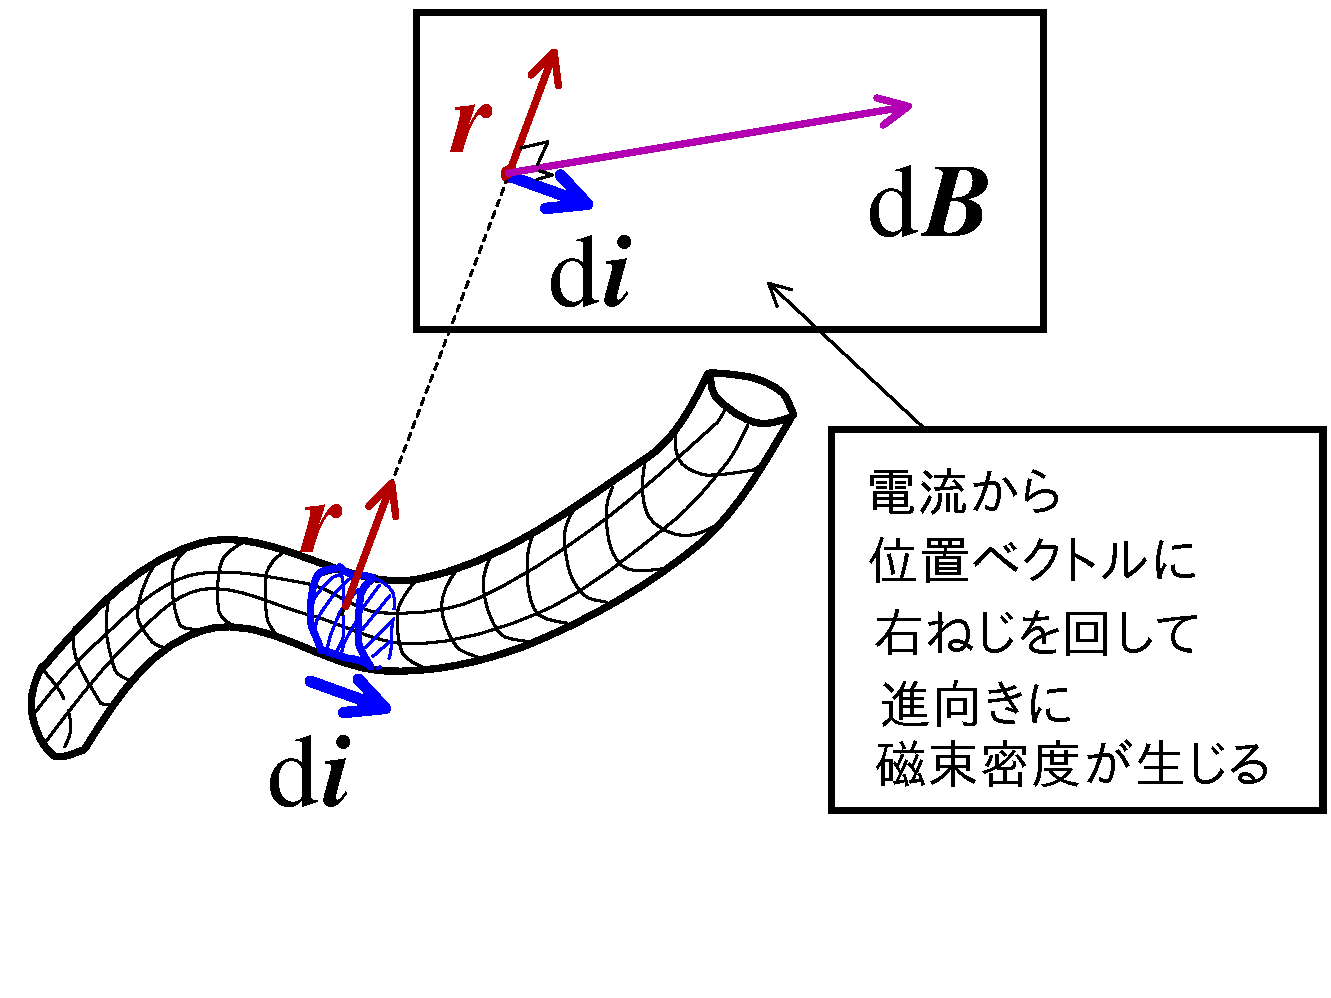
\includegraphics[keepaspectratio, width=7.2cm, height=5.79cm, clip]{biot_savart_1.pdf}
                    \caption{ビオ$=$サバールの法則}
                    \label{fig:biot_savart_1}
                \end{center}
            \end{figure}

    \subsection{点電荷の場合}
    最後に,電気量 $q$ をもつ点電荷に関する表示もしておこう.
    最初に示した式(\ref{Bior=savart'slow1})を思い起こそう.
        \begin{align*}
            \bB(\br)
            &=\frac{\mu_{0}|\bI|}{4\pi}
             \int_{\Gamma}\frac{\bt_{I}(\br')\times
                     (\br-\br')
                   }{|\br-\br'|^{3}}\df s' \\
            &=\frac{\mu_{0}}{4\pi}
             \int_{\Gamma}\frac{\bt_{I}(\br')\times
                     (\br-\br')
                    }{|\br-\br'|^{3}}|\bI|\df s'  \\
            \frac{\df \bB(\br)}{\df s'}
            &=\frac{\mu_{0}}{4\pi}
             \frac{\bt_{I}(\br')\times
                     (\br-\br')
                    }{|\br-\br'|^{3}}|\bI|  \\
            \df \bB(\br)
            &=\frac{\mu_{0}}{4\pi}
             \frac{\bt_{I}(\br')\times
                     (\br-\br')
                    }{|\br-\br'|^{3}}|\bI| \df s'  \\
            &=\frac{\mu_{0}}{4\pi}
             \frac{|\bI|\df s' \bt_{I}(\br')\times
                     (\br-\br')
                    }{|\br-\br'|^{3}}   \\
            &=\frac{\mu_{0}}{4\pi}|\bI|\df s' \bt_{I}(\br')\times
             \frac{(\br-\br')}{|\br-\br'|^{3}}
        \end{align*}

        ここで,\textbf{電流素片} という概念を導入しよう.
        上式の $|\bI|\df s' \bt_{I}(\br')$ に
        注目する.$\df s'$ は導線の微小な長さであるから,
        $|\bI|\df s' \bt_{I}(\br')$ という量は
        電流の微小な一部分であとみなせる.
        この $|\bI|\df s' \bt_{I}(\br')$ のことを電流素片と
        よぶことにしよう
            \footnote{
                教科書によっては,\textbf{電流要素} と表現されることもある.
            }.
        \begin{figure}[hbt]
            \begin{center}
                \includegraphicsdefault{dennryu_sohenn.pdf}
                \caption{電流素片 $|\bI|\df s \bt_{I}(\br)$}
                \label{fig:dennryu_sohenn}
            \end{center}
        \end{figure}


        電流素片 $|\bI| \df s'$ はその極限は,ひとつの点電荷の移動であると
        考えられる.点電荷の電気量を $q$,その速度を $\bv$ とすると,
        \begin{align*}
            |\bI| \df s' = q\bv.
        \end{align*}
        つまり,速度をもった点電荷が作る磁束密度 $\bB(\br)$ は
            \footnote{
                ここで,改めて,$\df \bB(\br)$ を $\bB(\br)$ に表示を置き換える.
                $\df \bB(\br)$ は電流の微小部分の作る磁束密度というイメージであったが,
                今考えている点電荷のつくる磁束密度であるので,それを $\bB(\br)$ と
                表現しても間違いではないだろう.いや,むしろこのように書き換えたほうが,
                式を自然な形にさせることができると思う.
            },
        \begin{align*}
            \bB(\br)
            &=\frac{\mu_{0}}{4\pi}q\bv \times
             \frac{\br-\br'}{|\br-\br'|^{3}}.
        \end{align*}
        \begin{myshadebox}{ビオ$=$サバールの法則(点電荷表示)}
            速度 $\bv$ で運動する,電気量 $q$ をもつ電荷は,次式で表される
            磁束密度 $\bB(\br)$ をその周囲に発生させる.
            \begin{align}
                \bB(\br)
                 &=\frac{\mu_{0}}{4\pi}q\bv \times
                  \frac{\br-\br'}{|\br-\br'|^{3}}.
            \end{align}
        \end{myshadebox}

